\documentclass{beamer}
\usetheme[titlepagelogo=minerva2,% Logo for the first page
						language=italian
                        ]{TorinoTh}
                        
\usepackage[beamer,customcolors]{hf-tikz}
\usepackage{verbatim}
\usepackage{algorithm}
\usepackage[noend]{algpseudocode}
\hfsetfillcolor{alerted text.fg!10}
\hfsetbordercolor{alerted text.fg}

\author{Marco Odore}
\rel{Prof. Giorgio Valentini}
\assistantsupervisor{Dr. Marco Notaro}
\title[Metodi di Ensemble Gerarchici]{Metodi di Ensemble Gerarchici per la Predizione Strutturata della Funzione delle Proteine}
\ateneo{Università Degli Studi Di Milano}
\date{10 Luglio 2018}

\begin{document}
\titlepageframe
\begin{tframe}{Central Dogma}
  % 
  \begin{columns}
    %
    \begin{column}{.65\textwidth}
      \minipage[c][0.4\textheight][s]{\columnwidth}
	   \begin{itemize}	
	  \item All'interno delle molecole di DNA di ogni essere vivente esistono diverse migliaia di geni.   
      \onslide<2->
	  \item Si stima che per l'essere umano il DNA possegga tra i 20.000 - 25.000 geni.
      \onslide<3->
      \item Ogni gene all'interno del DNA è capace di codificare più proteine.	
      \onslide<4->
      \item Ogni proteina è responsabile di una o più funzioni all'interno delle cellule degli esseri viventi.
      \end{itemize}
      \endminipage      
    \end{column}
    %
    \begin{column}{.35\textwidth}

      % for top aligned images use minipage
      \only<1-4>{
        \minipage[c][0.4\textheight][s]{\columnwidth}

        \onslide<1->    

        \only<1-4>{
          \begin{figure}
            \centering
            \includegraphics<1>[scale=0.2]{img/DNA.png} %         
            \includegraphics<2>[scale=0.3]{img/humandna.png} %
            \includegraphics<3>[scale=0.2]{img/centraldogma.png}%
            \includegraphics<4>[scale=0.5]{img/funzioni.jpg}
        \end{figure}}


        \endminipage
      }   

      % for vertically centered images use parbox

    \end{column}
  \end{columns}

\end{tframe}


\begin{tframe}{\small Il problema della predizione della funzione delle proteine 1/4}
  % 
  \begin{columns}
    %
    \begin{column}{.75\textwidth}
      \minipage[c][0.4\textheight][s]{\columnwidth}
	   \begin{itemize}	
	   \onslide<1->
	  \item L'individuazione della funzione delle proteine attraverso le analisi con sperimentazione diretta in laboratorio è \highlightbf{costosa} e richiede \highlightbf{molto tempo}
	  \onslide<2->
	  \item Esistono centinaia di funzioni a cui poter associare un gene/proteina \highlightbf{(problema multiclasse)}
	  \onslide<3->
	  \item Ad ogni gene/proteina possono essere associate diverse funzioni contemporaneamente \highlightbf{(problema multietichetta)}
      \onslide<4->
	  \item Il quantitativo di dati genomici cresce molto rapidamente.
      \end{itemize}
      \onslide<5->
      La \highlightbf{classificazione manuale} delle proteine è quindi infattibile.
      \endminipage      
    \end{column}
    %
    \begin{column}{.25\textwidth}

      % for top aligned images use minipage
      \only<1-5>{
        \minipage[c][0.4\textheight][s]{\columnwidth}

        \onslide<1->    

        \only<1-5>{
          \begin{figure}
            \centering
            \includegraphics<1>[scale=0.15]{img/lab3.jpg} %         
            \includegraphics<2>[scale=0.2]{img/multiclass.png} %
            \includegraphics<3>[scale=0.3]{img/multilabel.png}%
            \includegraphics<4->[scale=0.16]{img/growth.jpg}
        \end{figure}}


        \endminipage
      }   

      % for vertically centered images use parbox

    \end{column}
  \end{columns}

\end{tframe}

\begin{tframe}{\small Il problema della predizione della funzione delle proteine 2/4}
\begin{itemize}
\onslide<1->
\item A complicare ulteriormente il problema è il modo in cui sono \emph{relazionate} tra loro le funzioni delle proteine.
\onslide<2->
\item Esistono infatti due tassonomie principali per l'organizzazione delle classi:
\begin{itemize}

\onslide<3->
\item \highlightbf{Gene Ontology} (GO):  che organizza le funzioni come un grafo diretto aciclico (DAG), varia per ogni specie, e possiede tre ontologie differenti.
\onslide<4->
\item \highlightbf{Functional Catalogue} (FunCat): che è organizzato invece come un albero, non varia in base alle specie, e descrive le funzioni in maniera più sintetica rispetto alla Gene Ontology.
\end{itemize}

\end{itemize}  

\end{tframe}
\begin{tframe}{\small Il problema della predizione della funzione delle proteine  3/4}
\begin{figure}[h]
\center
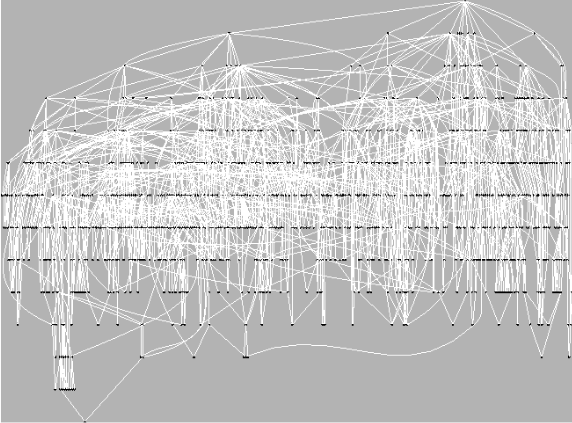
\includegraphics[scale=0.25]{./img/GO.png}
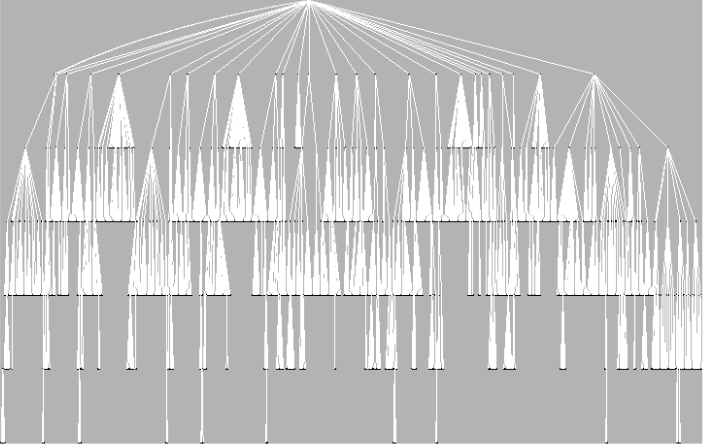
\includegraphics[scale=0.24]{./img/FunCat.png}
\caption{\footnotesize{A sinistra un DAG della GO per la specie \emph{S. cerevisiae}. A destra FunCat.}}
\label{DAGTREE}
\end{figure}
\end{tframe}


\begin{tframe}{\small Il problema della predizione della funzione delle proteine (GO) 4/4}
\begin{itemize}
\onslide<1->
\item Data la granularità e specificità superiori della GO e il suo largo utilizzo nella comunità scientifica, all’interno della tesi ci si è soffermati sulla predizione delle sue funzioni.
\onslide<2->
\item Tale tassonomia presenta tre ontologie (e quindi tre DAG) principali:
\begin{itemize}
\onslide<3->
\item \highlightbf{Processo Biologico} (BP): descrive i processi ad alto livello, come insieme di diverse attività molecolari.
\onslide<4->
\item \highlightbf{Funzione Molecolare} (MF): descrive le funzioni di specifici prodotti genici.
\onslide<5->
\item \highlightbf{Componente Cellulare} (CC): il luogo all’interno della cellula nelle quali avviene la funzione genica.
\end{itemize}
\end{itemize}  

\end{tframe}



\begin{tframe}{\footnotesize{La predizione della funzione delle proteine tramite metodi automatici}}
Per gestire il problema della predizione della funzione delle proteine si rende quindi necessario un approccio \highlightbf{automatico}. I metodi più noti in letteratura sono:

\begin{itemize}
\onslide<2->
\item I metodi basati sulla \highlightbf{comparazione di biosequenze}: si basano sull'idea che sequenze simili condividano funzioni simili.
\onslide<3->
\item I metodi \highlightbf{basati su reti}: sono metodi applicati a dati rappresentati sotto forma di reti, che si basano sugli algoritmi di propagazione delle etichette.
\onslide<4->
\item I metodi \highlightbf{Kernel per spazi di output strutturato}: sono metodi che sfruttano funzioni kernel congiunte per predire in spazi di output strutturato.
\onslide<5->
\item I metodi \highlightbf{Ensemble Gerarchici}: i metodi trattati in questa tesi.
\end{itemize}

\end{tframe}

\begin{tframe}{Metodi Ensemble Gerarchici 1/3}
I Metodi di Ensemble Gerarchici sono metodi caratterizzati da due step principali:

\begin{enumerate}
\onslide<2->
\item \highlight{Predizione flat} delle diverse classi dell’ontologia, generando diversi predittori \emph{indipendenti}.
\onslide<3->
\item \highlight{Combinazione e correzione gerarchica delle predizioni} sfruttando il DAG dei termini della GO.
\end{enumerate}
\onslide<4->
Il secondo step rappresenta la componente \emph{ensemble} del metodo. Tale step si rende necessario in quanto le predizioni flat non tengono in considerazione la struttura gerarchica dei DAG della GO, portando a risultati \emph{inconsistenti}.

\end{tframe}
\begin{tframe}{Metodi Ensemble Gerarchici 2/3} 

\block{Consistenza \& True Path Rule}
Un insieme di predizioni $\hat{y} = <\hat{y}_1, \hat{y}_2, \dots, \hat{y}_{|N|}>$, dove $|N|$ è la cardinalità dei termini della gerarchia, è definito \emph{consistente}, se rispetta la \emph{True Path Rule}, e cioè:
\[
y\;\;\;consistente\;\; \leftrightarrow \forall i \in N, j \in par(i) \rightarrow y_j \geq y_i
\] 
Dove $par(i)$ indica l'insieme dei termini genitori del nodo $i$ nella gerarchia.
\endblock{}
\end{tframe}
\begin{tframe}{Metodi Ensemble Gerarchici (Esempio) 3/3}

\begin{center}
\includegraphics<1>[width=5cm]{img/1_1.png}
\includegraphics<2>[width=5cm]{img/2.png}
\includegraphics<3>[width=5cm]{img/3.png}
\includegraphics<4>[width=8.22cm]{img/4.png}
\end{center}
%\caption{Predittori flat indipendenti}


\end{tframe} 

\begin{tframe}{Metodi Ensemble Gerarchici: Approcci}
\begin{columns}
    \begin{column}{.50\textwidth}
      \minipage[c][0.4\textheight][s]{\columnwidth}
      Esistono fondamentalmente due approcci per la correzione:
	   \begin{itemize}
	   \onslide<2->
	  \item \highlight{Top-down}: le predizioni vengono corrette dai nodi più generali a quelli più specifici.
	   \onslide<3->	  
	  \item \highlight{Bottom-up}: Le predizioni vengono corrette dai nodi più specifici verso quelli più generali.
      \end{itemize}
      \endminipage 
    \end{column}
    %
    \begin{column}{.50\textwidth}
    \onslide<2-> 
        \minipage[c][0.4\textheight][s]{\columnwidth}
        \only<2-3>{
          \begin{figure}
            \centering
            \includegraphics<2>[scale=0.3]{img/topdown.png}
            \includegraphics<3>[scale=0.3]{img/bottomup.png}
        \end{figure}}
        \endminipage
    \end{column}
  \end{columns}
\end{tframe}

\begin{tframe}{Metodo Top-Down Gerarchico (HTD-DAG)}
\begin{itemize}

\onslide<1->
\item È un metodo che utilizza l'approccio \emph{Top-Down}.
\onslide<2->
\item La correzione avviene ricorsivamente, percorrendo il grafo per \emph{livelli}. Più precisamente, dato il grafo $G = (N, E)$, gli score flat $f(x) = \hat{y}$ sono corretti gerarchicamente a $\bar{y}$, applicando la seguente regola:
\begin{block}{Aggiornamento con HTD-DAG}
\[
\bar{y}_i := 
\begin{cases}
\hat{y}_i \;\;\;\;\;\;\;\;\;\;\;\;\;\;\;\;\;\;\;\;\; if\;\; i \in root(G)\\
min_{j \in par(i)} \bar{y}_j \;\;\;\; if \;\; min_{j \in par(i)}\bar{y}_j < \hat{y}_i\\
\hat{y}_i \;\;\;\;\;\;\;\;\;\;\;\;\;\;\;\;\;\;\;\;\; altrimenti
\end{cases}
\]
\end{block}
Dove $par(i)$ specifica i genitori del nodo $i$.
\end{itemize} 
\end{tframe}

\begin{tframe}{Metodo True Path Rule per DAG (TPR-DAG)}
\begin{itemize}
\onslide<1->
\item È un metodo che combina gli approcci top-down e bottom-up per la correzione delle predizioni flat. 
\onslide<2->
\item È suddiviso in due step sequenziali:
\begin{enumerate}
\onslide<3->
\item \highlightbf{Step bottom-up}: che partendo dai nodi più specifici del DAG, propaga quelle predizioni flat che sono considerate \highlight{positive}.
\onslide<4->
\item \highlightbf{Step top-down}: È il medesimo step utilizzato dal metodo HTD-DAG.
\end{enumerate}
\onslide<5->
\item Lo step top down si rende necessario in quanto la propagazione delle predizioni positive dal basso verso l’alto non garantisce la consistenza delle predizioni necessarie alla True Path Rule. 
\end{itemize}
\end{tframe}

\begin{comment}
\begin{tframe}{Metodo True Path Rule per DAG (TPR-DAG) (2/2)}
\begin{itemize}
\onslide<1->
\item Entrando nel dettaglio dello step bottom-up, data una predizione $\hat{y}_{i}$ per il nodo $i \in N$, questa viene aggiornata come:
\begin{block}{Aggiornamento step Bottom-up TPR-DAG}
\[
\bar{y}_i = \frac{1}{1 + |\phi_i|} (\hat{y}_i + \sum_{j \in \phi_i} \bar{y}_j)
\]
\end{block}
Dove $\phi_i$ rappresenta l'insieme dei figli del nodo $i$ che sono considerati \emph{positivi} in relazione alla predizione.
\end{itemize}
\end{tframe}
\end{comment}

\begin{comment}
\begin{tframe}{Metodo True Path Rule per DAG (TPR-DAG) 3/3}
\begin{itemize}
\onslide<1->
\item L'insieme $\phi$ dei \emph{positivi} può essere generato in diversi modi:
\begin{enumerate}
\onslide<2->
\item \highlight{senza soglia}: I figli selezionati sono quelli che hanno un valore per la predizione superiore a quello del genitore
\onslide<3->
\item \highlight{soglia costante}: I figli sono considerati positivi se le predizioni superano una soglia (es. 0.5).
\onslide<4->
\item \highlight{soglia adattiva}: La soglia per selezionare i figli si ottiene tramite il tuning con massimizzazione di una metrica. 
\end{enumerate}
\onslide<5->
\item Oltre a questi tipi di selezione, possono essere introdotti in combinazione dei pesi $w$, trasformando l'aggiornamento come:
\begin{block}{Aggiornamento step Bottom-up TPR-DAG con $w$}
\[
\bar{y}_i = w \hat{y}_i + \frac{(1-w)}{|\phi_i|}\sum_{j \in \phi_i}\bar{y}_j
\]
\end{block}
\end{itemize}
\end{tframe}
\end{comment}

\begin{tframe}{Generalized Pool Adjacent Violator (GPAV) (1/4)}
\begin{itemize}
\onslide<1->
\item Per il passo Top-Down dell’algoritmo TPR-DAG (e HTD) è possibile sfruttare gli algoritmi per la risoluzione dei problemi di \highlightbf{Isotonic Regression}:
\begin{block}{Isotonic Regression (caso generale con ordinamento parziale)}
Dato un DAG, $G(N, E)$, con il set di nodi $N = \{1, 2, ..., n\}$, si deve trovare il vettore $x^{*}\in R^{n}$ tale che:
\[
min \sum_{i=1}^{n} w_i (x_i - a_i)^2
\]
\begin{center}
such that $x_i \le x_j$ $\forall (i,j) \in E $ 
\end{center}
\end{block} 

\end{itemize}
\end{tframe}
\begin{tframe}{Generalized Pool Adjacent Violator (GPAV) (2/4)}
Esempio di Isotonic Regression con \emph{ordinamento totale}:
\begin{figure}
\centering
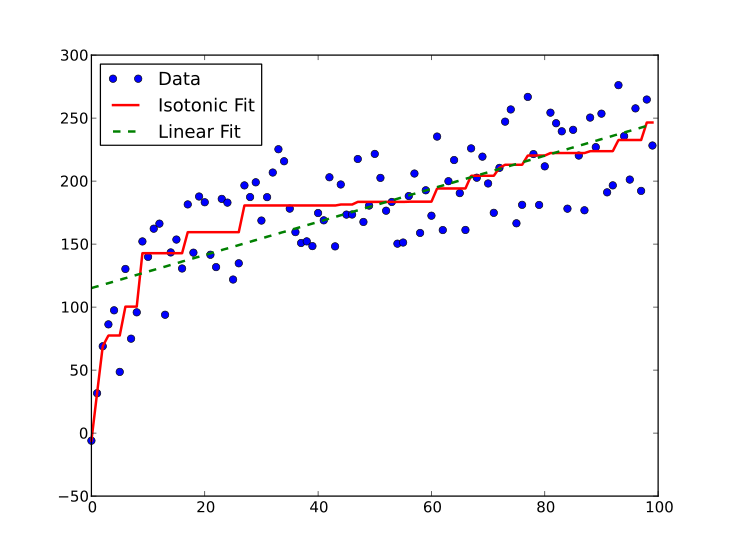
\includegraphics[scale=0.3]{img/monotonic.png}
\end{figure}
\end{tframe}
\begin{tframe}{Generalized Pool Adjacent Violator (GPAV) (3/4)}
Funzionamento Generale:
\begin{itemize}
\onslide<2->
\item Per far funzionare l'algoritmo è necessario effettuare un \highlight{ordinamento topologico} del grafo.
\onslide<3->
\item L’algoritmo genera uno split del set di nodi $N$ del DAG, in un insieme di \highlight{blocchi disgiunti definiti da $H$} (inizialmente $H = N$).
\onslide<4->
\item Seguendo l'ordinamento topologico del grafo, un blocco \highlight{assorbe} un suo blocco \emph{predecessore} se si verificano determinate condizioni.
\onslide<5->
\item I nodi presenti nel medesimo blocco $B_i$ \highlight{condividono il medesimo valore} $x_i$, e quindi a seguito dell'assorbimento sarà necessario un aggiornamento di tale valore.
\end{itemize}
\end{tframe}

\begin{comment}
\begin{tframe}{Generalized Pool Adjacent Violator (GPAV) (4/5)}
La procedura di assorbimento:
\begin{center}
\scalebox{0.85}{
\begin{minipage}{0.9\linewidth}
\begin{algorithm}[H]
\caption{Absorb}\label{ABSORB}
\begin{algorithmic}[1]
\Procedure{Absorb($j, i$)}{}
\State $ H = H \backslash \{i\} $
\State $ B_j^{-} = B_i^{-}\cup B_j^{-}\backslash \{i\} $
\State $x_j = \frac{W_j x_j + W_i x_i}{W_j + W_i}$
\State $B_j = B_j \cup B_i$
\State $W_j = W_j + W_i$
\For{(each $k \in H\;\; s.t.\;\; i  \in B_k^{-} $)}
\State $B_k^{-} = B_k^{-}\backslash \{i\} \cup \{j\}$ 
\EndFor
\EndProcedure
\end{algorithmic}
\end{algorithm}
\end{minipage}}
\end{center}
\end{tframe}
\end{comment}

\begin{tframe}{Generalized Pool Adjacent Violator (GPAV) (4/4)}

\begin{center}
\scalebox{0.85}{
    \begin{minipage}{0.9\linewidth}
\begin{algorithm}[H]

\caption{GPAV}\label{gpav}
\begin{algorithmic}[1]
\Procedure{GPAV}{}
\State $ H = N $
\For{(each $i \in N$)}
\State $B_i = \{i\}$ 
\State $B_i^{-} = i^{-}$
\State $x_i = \hat{y}_i$
\State $W_i = w_i$
\EndFor
\For{$k = 1, 2, ..., n$}
\State \footnotesize{\emph{//finché esiste un predecessore di $B_{k}$ che viola la monotonicità}}
\While{$\{i \in B_k^{-}: x_i > x_k\}\neq 0$} 
\State \footnotesize{\emph{// Trova l'elemento che viola maggiormente il vincolo}}
\State \textbf{Find} $j \in B_k^{-}: x_j = max\{x_i : i \in B_k^{-}\}$ 
\State \textbf{Absorb(k, j)} \emph{// $j$ viene assorbito da $B_k$}
\EndWhile
\EndFor
\EndProcedure
\end{algorithmic}
\end{algorithm}
\end{minipage}}
\end{center}
\end{tframe}
\begin{tframe}{Metodi GPAV e ISO-TPR}
\begin{itemize}
\onslide<1->
\item Riassumendo, l’algoritmo effettua degli assorbimenti di blocchi adiacenti, finché questi violano i vincoli del problema quadratico, generando di fatto una partizione dei nodi, in cui le parti condividono lo stesso valore.
\onslide<2->
\item L'algoritmo GPAV ha una complessità pari a $O(n^2)$.
\onslide<3->
\item Sostituendo quindi GPAV allo step Top-Down dell'algoritmo TPR-DAG visto in precedenza (invece che HTD), si ottiene l'algoritmo ISO-TPR.
\end{itemize}

\end{tframe}
\begin{tframe}{\footnotesize{Predizione della funzione delle proteine della specie C.elegans (WORM) 1/4}}
Il dataset del nostro problema:
\begin{itemize}
\onslide<2->
\item Si è eseguita la sperimentazione sul genoma della specie
\highlight{Caenorhabditis elegans} (WORM), un organismo modello molto semplice, utilizzato frequentemente in biologia, soprattutto per studi di biologia dello sviluppo.
\onslide<3->
\item L’insieme delle istanze utilizzato come input dai diversi predittori per il nostro problema, è dato dall’insieme dei geni della specie oggetto della sperimentazione, il quale è rappresentato da una matrice simmetrica generata dal network di interazione proteina-proteina estratto dal database \highlight{STRING} (Search Tool for the Retrieval of Interacting Genes/Proteins).
\end{itemize}
\end{tframe}

\begin{comment}
\begin{tframe}{\footnotesize{Predizione della funzione delle proteine della specie C.elegans (WORM)} 2/4}
\begin{figure}
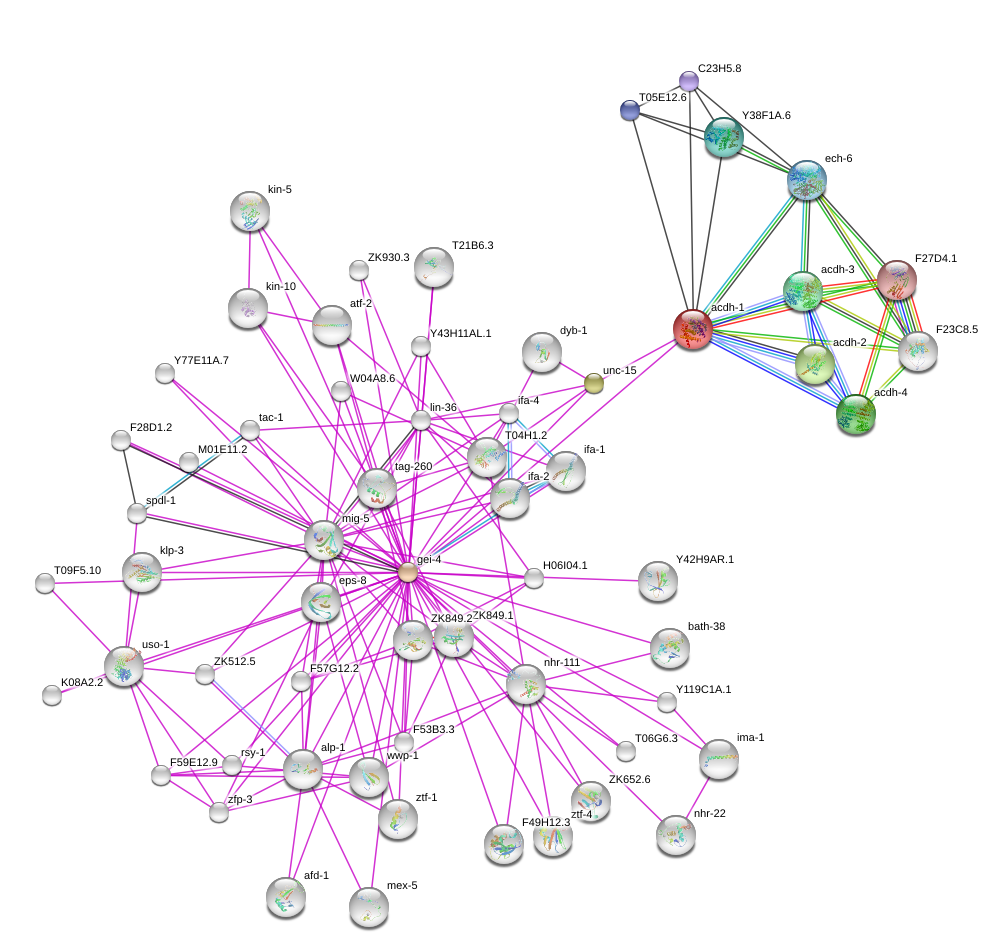
\includegraphics[scale=0.2]{img/STRING-NET.png}
\caption{\footnotesize{Una porzione del grafo STRING per la specie WORM.}}
\end{figure}
\end{tframe}
\begin{tframe}{\footnotesize{Predizione della funzione delle proteine della specie C.elegans (WORM)} 3/4}
Cosa indicano le relazioni tra proteine in STRING:
\begin{itemize}
\onslide<2->
\item Le interazioni proteiche verificate sperimentalmente, presenti in database
primari.
\onslide<3->
\item Le informazioni del pathway 4 ottenute da database curati.
\onslide<4->
\item I collegamenti semantici e/o statistici fra le proteine, ottenuti dall’analisi effettuata tramite text-mining.
\onslide<5->
\item Le interazioni ottenute tramite diversi algoritmi sulle informazioni genetiche.
\onslide<6->
\item Le interazioni dei geni ortologhi, e cioè geni che sono presenti in specie diverse ma correlate, che codificano per proteine con strutture e funzioni simili.
\end{itemize}
\onslide<7->
Questi score combinati proteina-proteina rappresentano di fatto le feature (o caratteristiche) delle istanze.
\end{tframe}
\end{comment}

\begin{tframe}{\footnotesize{Predizione della funzione delle proteine della specie C.elegans (WORM)} 4/4}
Un po' di info sul dataset:
\begin{itemize}
\onslide<2->
\item Nel caso specifico della specie C.elegans, la matrice STRING ha dimensione 15752×15752. Il nostro problema ha quindi 15752 istanze.
\onslide<3->
\item Per le classi funzionali/termini e annotazioni, queste cambiano in base al DAG di riferimento:
\begin{table}[h]
\centering
\begin{tabular}{|l|l|l|}
\hline
      \textbf{ ontologia} & \textbf{numero di termini} & \textbf{numero di archi} \\ \hline
BP & 4068  &  8066   \\ 
\hline
MF  & 1163  & 1567   \\ 
\hline
CC  & 578  & 1082     \\ 
\hline
\end{tabular}
\caption{\footnotesize{Statistiche relative ai DAG delle annotazioni della specie C.elegans.}}
\label{DAG_desc}
\end{table}

\end{itemize}
\end{tframe}

\begin{tframe}{\footnotesize{Predizione della funzione delle proteine della specie C.elegans (WORM)} 4/4}

Per evitare di avere problemi nella cross-validazione, i DAG sono stati ridotti a quei termini per cui si hanno almeno 10 annotazioni. Un po' di statistiche a seguito della selezione:
\begin{table}[h]
\centering
\begin{tabular}{|l|l|l|l|l|l|}
\hline
\textbf{Onto} & \textbf{numero di termini} & \textbf{media} & \textbf{d.std.} & \textbf{massimo} & \textbf{minimo} \\ \hline
BP            & 1335                & 71,33                & 151,68              & 2597                & 10                  \\ \hline
MF            & 186                 & 61,23                & 191,84              & 1806                & 10                  \\ \hline
CC            & 221                 & 131,9                & 302,25              & 1924                & 10                  \\ \hline
\end{tabular}
\caption{\footnotesize{La colonna \emph{numero di termini} indica il numero di termini ottenuti dopo la selezione, \emph{media} la media delle annotazioni per classe, per l'ontologia di riferimento, \emph{d.std.} la deviazione standard delle annotazioni per l'ontologia di riferimento, \emph{massimo} e \emph{minimo} rispettivamente il massimo e minimo numero di annotazioni.}}
\label{riduzioneann}
\end{table}
\end{tframe}
\end{document}
